\documentclass{beamer}
% \usepackage{animate}
\usepackage{multimedia}

\usepackage{pgfpages}
\setbeameroption{show notes on second screen}
%https://tug.ctan.org/macros/latex/contrib/beamer/doc/beameruserguide.pdf

\usepackage[T2A]{fontenc}
\usepackage[utf8]{inputenc}
\usepackage[english,russian]{babel}
\usepackage{amsmath}
\usepackage{textcomp}
% \usepackage{hyperref}
% \usepackage{bookmark}
\hypersetup{unicode=true}

\setbeamertemplate{caption}[numbered]

\usetheme{CambridgeUS}
\usecolortheme{dolphin}


\title[Отсев]{Отсев (Culling)}
\author[Быковских Д.А.]{Быковских Дмитрий Александрович}
\date{18.10.2025}

\begin{document}
	\begin{frame}
		\titlepage
	\end{frame}

	\begin{frame}{Culling}

		В современных видеоиграх и приложениях реального времени сцены могут содержать тысячи или даже миллионы объектов. Без отсечения система будет пытаться рендерить все объекты, даже если большая часть из них не видна. Это значительно замедлит процесс рендеринга и снизит производительность.
		

		\textbf{Culling (c англ. отсев, отбор, выборка) --- процесс оптимизации рендеринга, суть которого заключается в исключении невидимых объектов в кадре, с целью экономии вычислительных ресурсов.}



		Отсев (Culling) позволяет уменьшить нагрузку на центральный и графический процессоры, избегая рендеринга ненужных объектов. Это особенно критично для игр с большими открытыми мирами, таких как RPG или FPS, где игрок перемещается по огромным пространствам с множеством объектов.

		\note{
			\begin{figure}
				\href{https://www.simbasible.com/far-cry-game-review/}{
					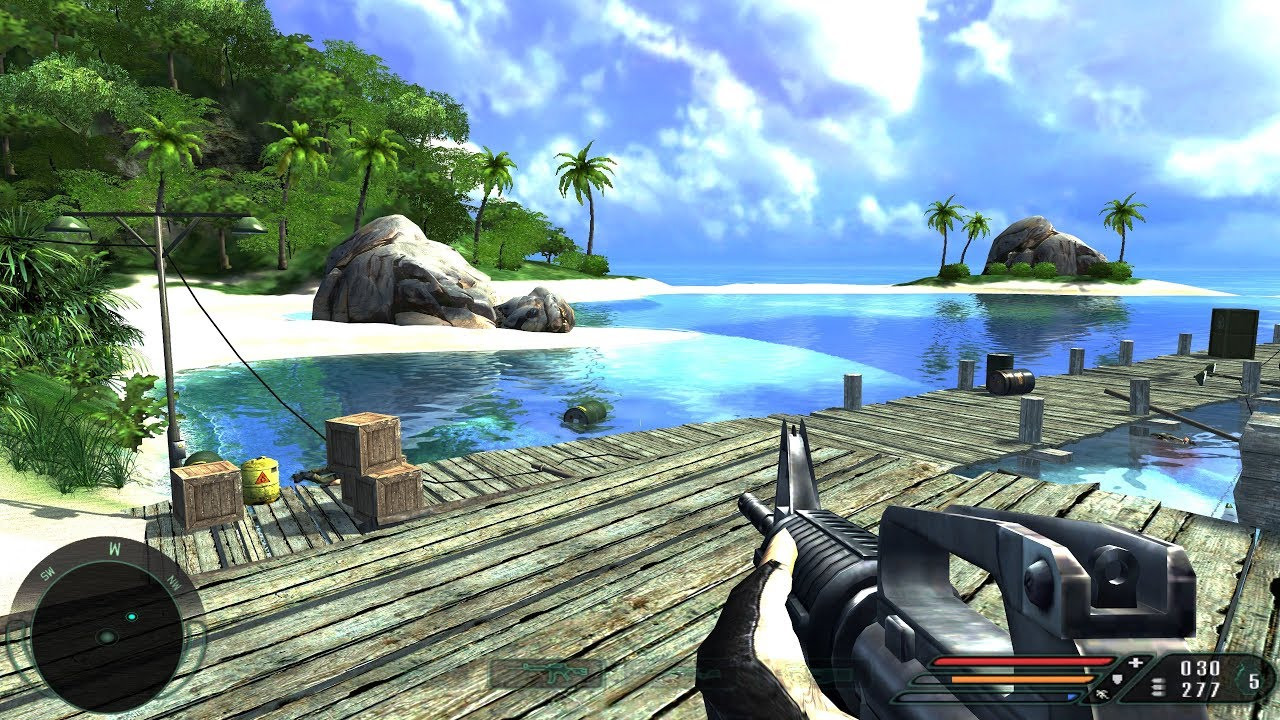
\includegraphics[width=0.95\textwidth]{images/FarCry-2004.jpg}}
				\caption {Открытый мир в игре Far Cry (2004 г.)}
			\end{figure}
		}

	\end{frame}

	\begin{frame}{Этапы c применением отсева}
		\begin{itemize}
			\item 			
			Geometric stage (Геометрический этап). Отсев начинается с анализа сцены, где объекты проверяются на видимость относительно камеры. \\ Frustum Culling и Portal Culling применяются на этом этапе.
			\item 
			Rasterization stage (Этап растеризации). 
			Позволяет исключить полигоны (поверхности), нормаль которых направлена от камеры (или к камере). \\
			Этот этап включает Face Culling. 
			\item 
			Pixel stage (Этап обработки пикселей). Применяется, когда
			пиксели уже предварительно обработаны, если объекты перекрываются другими. Аппаратные и программные методы позволяют сделать это на уровне GPU, что помогает избежать затрат на рендеринг окклюдированных объектов. \\
			На этом этапе применяется Occlusion Culling.
		\end{itemize}

	




		\note {

		Комплексные техники и оптимизации (требующие дополнительных вычислений) \\
		Hierarchical Culling (Иерархический отсев)
		и  
		Level of Detail (LOD) 

		% 	Инструменты и библиотеки

		% 	Реализация методов отбора зависит от графического движка или программной библиотеки, которая используется для рендеринга. Например:
		% 	\begin{itemize}
		% 		\item 	
		% 		В DirectX и OpenGL есть встроенные функции для Face Culling и другие механизмы отбора.
		% 		\item 
		% 		Unity и Unreal Engine предоставляют встроенные методы для Frustum и Occlusion Culling.
		% 		\item 
		% 		Umbra — это коммерческая библиотека, которая оптимизирует occlusion culling и масштабные сцены.
		% 	\end{itemize}
		}
	\end{frame}

	\begin{frame}{Geometric stage. Frustum Culling}{Отсев по пирамиде видимости}

	Простая идея. Если камера смотрит прямо, все объекты за спиной камеры будут исключены из обработки.

	\textbf{Пирамида видимости (frustum)} --- объём пространства, который видит камера в 3D-пространстве. Всё, что находится за пределами этой пирамиды, не будет видно в кадре.

	\textbf{Frustum Culling} --- процесс, при котором объекты, находящиеся за пределами пирамиды видимости камеры, исключаются из рендеринга. Это один из самых простых и эффективных методов отсечения.


	\note{
		\begin{figure}
			\href{https://www.gamedev.net/tutorials/programming/general-and-gameplay-programming/frustum-culling-r4613/}{
					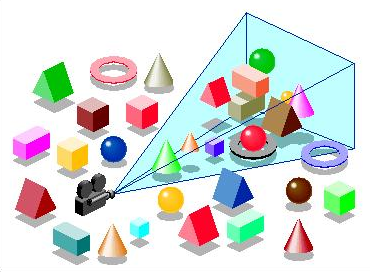
\includegraphics[width=0.46\textwidth]{images/frustum-culling-1.png}
			}
			\href{https://www.gamedev.net/tutorials/programming/general-and-gameplay-programming/frustum-culling-r4613/}{
					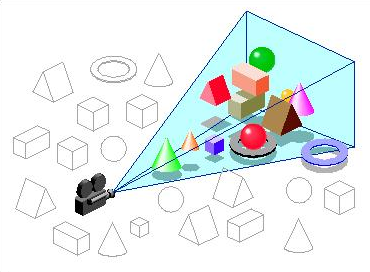
\includegraphics[width=0.46\textwidth]{images/frustum-culling-2.png}
			}
			\caption{Отсев по пирамиде видимости: до (слева) и после (справа)}
		\end{figure}
	}

	\end{frame}

	\begin{frame}{Geometric stage. Portal Culling}{Отсев через порталы}
		
		\textbf{Portal Culling} --- метод, применяемый в сценах, которые делятся на секции или комнаты, соединенные «порталами» (двери, окна и т.д.). Если камера не может видеть через портал, то объекты, находящиеся в другой комнате, будут исключены. Этот метод часто используется в играх, где игрок перемещается между различными областями, например, в зданиях или туннелях.
		
		\vspace{0.5cm}
		Пример. \\ 
		Пусть дана сцена квартиры, с заполненными комнатами. \\
		Задача. Исключить объекты, находящиеся вне зоны видимости, т.е. за порталами (двери, окна).\\
		Например, если дверь в другую комнату закрыта, сцена внутри другой комнаты может быть исключена из рендеринга. \\
				
		\note{
			Основное предназначение этого метода заключается в оптимизации отрисовки игр с архитектурными сценами.

			\begin{figure}
				\href{https://www.simbasible.com/far-cry-game-review/}{
					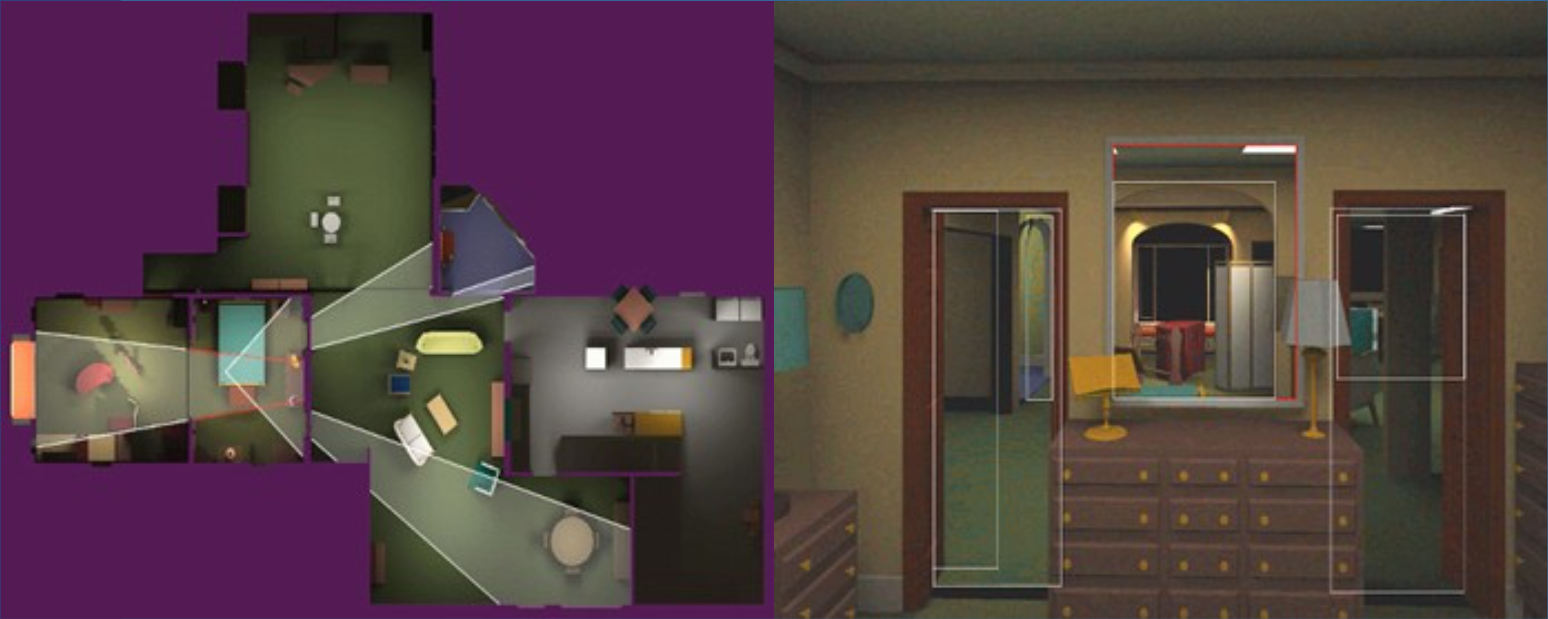
\includegraphics[width=1.0\textwidth]{images/portal-culling.png}}
				\caption {Portals and Mirrors, David P. Luebke and Chris Georges}
			\end{figure}
		}

	\end{frame}

	\begin{frame}{Rasterization stage. Face Culling}{Исключение граней}

		Face culling (исключение граней) --- более общий термин, который описывает процесс исключения каких-либо (например, обратных или лицевых) граней (полигонов) объекта из рендеринга.
		
		Backface culling (исключение обратных граней) --- техника, которая исключает из рендеринга задние (обратные) грани трёхмерных объектов. Эти грани считаются невидимыми для зрителя, так как они направлены в противоположную от камеры сторону.
	
		{ \footnotesize
		Описание Backface culling:
		\begin{itemize}
			\item 	
			Трёхмерные объекты обычно состоят из полигонов (чаще всего треугольников), которые часто рассматриваются как однонаправленные поверхности.
			\item 
			Каждый треугольник имеет нормаль (вектор, перпендикулярный поверхности).
			\item 
			Если нормаль треугольника направлена от камеры (т.е. обратная сторона полигона), этот треугольник считается невидимым и исключается из рендеринга.
		\end{itemize}

		% Пример. \\
		% Если вы смотрите на внешнюю сторону куба, полигоны, которые находятся внутри куба или «смотрят» в его сторону, будут исключены.
		
		}

		\note{

			\begin{figure}
				\href{https://learnopengl.com/Advanced-OpenGL/Face-culling/}{
						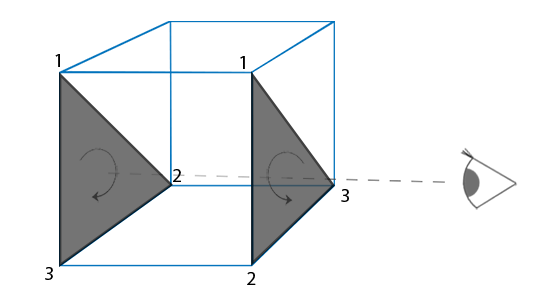
\includegraphics[width=0.46\textwidth]{images/faceculling-frontback.png}
				}
				\href{https://web.archive.org/web/20010206194247/http://thesims.ea.com/us/}{
						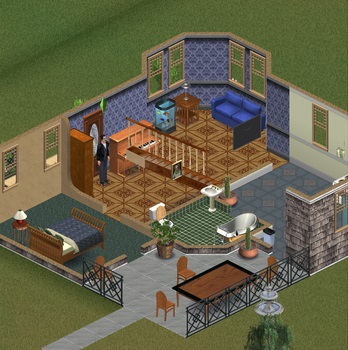
\includegraphics[width=0.46\textwidth]{images/the-sims.jpg}
				}
				\caption{Face culling: для куба, состоящего из треугольников (слева) и применение техники в игровой сцене The Sims (справа)}
			\end{figure}

		}

	\end{frame}

	\begin{frame}{Pixel stage. Occlusion Culling}{Отсев по окклюзии}

Этот метод отсечения удаляет из рендеринга объекты, которые перекрыты другими объектами и полностью скрыты от камеры. 
\\
Например, если за зданием находится дерево, и здание полностью его закрывает, дерево можно исключить из рендеринга. 
\\
Occlusion Culling работает с учетом геометрии сцены, рассчитывая, какие объекты скрыты за другими.

\vspace{0.5cm}
Пример. \\
Стоя перед зданием, камера не увидит объекты, находящиеся за ним. Тогда можно не тратить вычислительные ресурсы на отрисовку этих объектов, так как они не повлияют на кадр.

\note{

\begin{figure}
	\href{http://archive.gamedev.net/archive/reference/programming/features/occlusionculling/index.html}{
			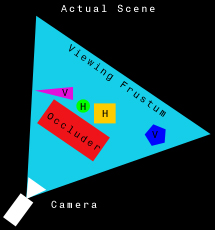
\includegraphics[width=0.4\textwidth]{images/occlusion-culling-scene.jpg}
	}
	\href{http://archive.gamedev.net/archive/reference/programming/features/occlusionculling/index.html}{
			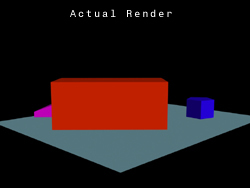
\includegraphics[width=0.55\textwidth]{images/occlusion-culling-render.jpg}
	}
	\caption{Occlusion culling: пример сцены (слева) и результат работы (справа)}
\end{figure}

}

	\end{frame}



	\begin{frame}{Hierarchical Culling }{Иерархический отсев}
		
		Hierarchical Culling --- оптимизация рендеринга путём исключения невидимых объектов на основе их положения и иерархической структуры.

		% Использование иерархии объектов для быстрого определения, какие объекты или группы объектов находятся вне поля зрения и могут быть исключены из обработки.

		Основные этапы:
		\begin{itemize}
			\item 	
			Построение иерархической структуры объектов сцены.
			\begin{itemize}
				\item 
				Bounding Volume. Каждая группа объектов оборачивается в объёмный контейнер (сферу или прямоугольный параллелепипед, AABB), который проверяется на пересечение с camera frustum камеры.
				\item 
				Иерархическая структура. Объекты группируются в древовидную структуру (например, Bounding Volume Hierarchy, BVH).
			\end{itemize}
			\item 
			Рекурсивный отсев при отрисовке сцены. Если объём не пересекается с frustum, вся группа объектов исключается. Если пересекается, проверяются дочерние объекты.
		\end{itemize}
	
		{
			\footnotesize
			Примечание. 
			AABB (Axis-Aligned Bounding Box) --- прямоугольный ограничивающий объём, выровненный по осям координат.
		}

		\note{
			\begin{figure}
				\href{https://learnopengl.com/Guest-Articles/2021/Scene/Frustum-Culling}{
					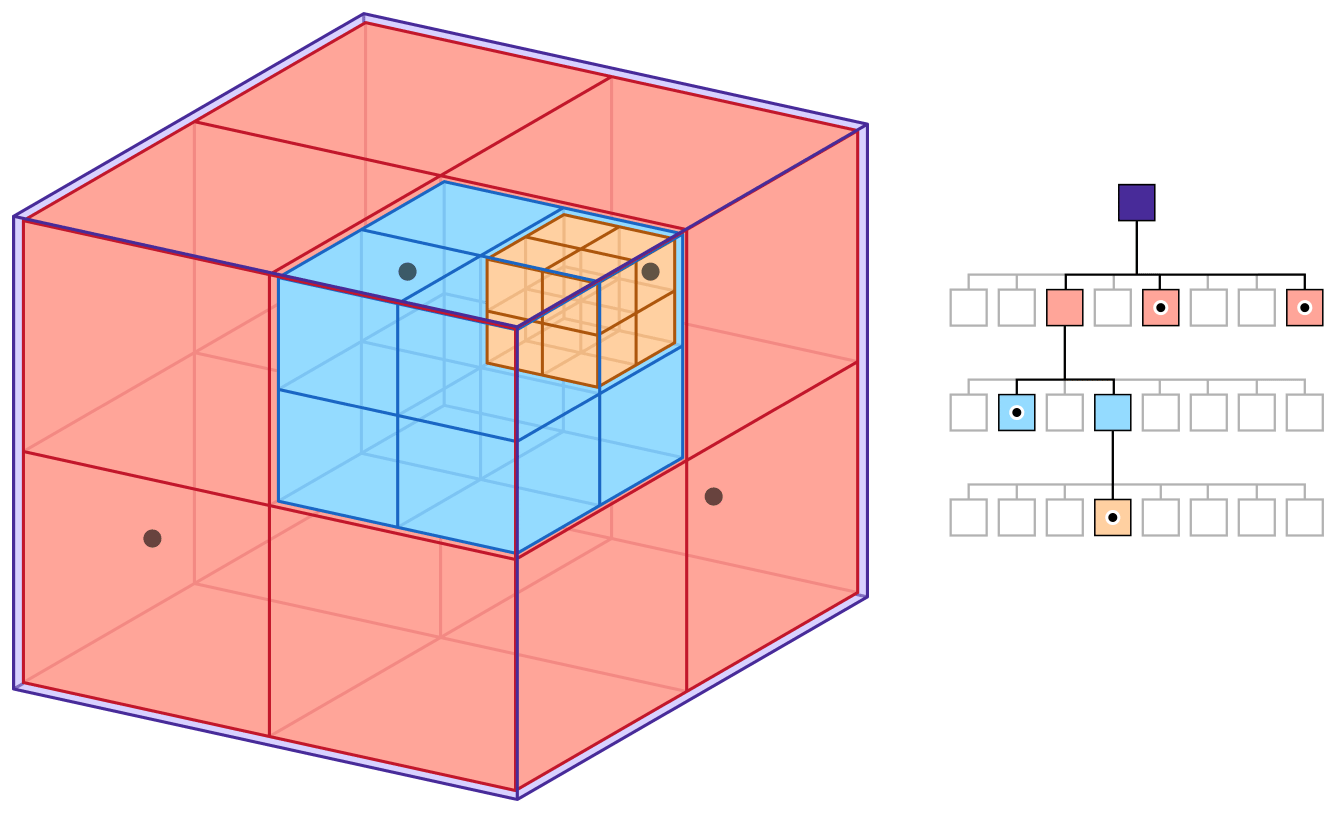
\includegraphics[width=0.8\textwidth]{images/octree.png}}
				\caption {Визуализация схемы пространственного разделения и структура октодерева (Octree)}
			\end{figure}
		}

	\end{frame}

	\begin{frame}{Level of Detail (LOD)}{Уровень детализации}
		Level of Detail (уровень детализации) не является прямым видом отсечения, хотя часто используется вместе с отсевом для оптимизации рендеринга. 

		LOD (Level of Detail) --- техника, при которой объекты рендерятся с меньшей детализацией, если они находятся далеко от камеры. Таким образом, уменьшается количество полигонов, обрабатываемых для удалённых объектов, сохраняя ресурсы.

		{ \footnotesize

		Примечание. \\
		Level of Development (уровень разработки) --- термин, используемый в архитектуре и строительстве, особенно в контексте информационного моделирования зданий (Building Information Modeling, BIM). Он описывает степень проработки и детализации объектов модели в различных стадиях проектирования и строительства.

		Mipmap (Multum In Parvo, Многое в малом) представляет собой предварительно созданный набор (иерархию) изображений, где каждое последующее изображение в этом наборе имеет размер в половину (или в другой пропорции) меньший, чем предыдущее.
		
		\\

		}

		\note{
			\begin{figure}
				\href{https://www.researchgate.net/publication/279847360_Coupling_of_CityGML-based_semantic_city_Models_with_energy_simulation_tools_some_experiences}{
					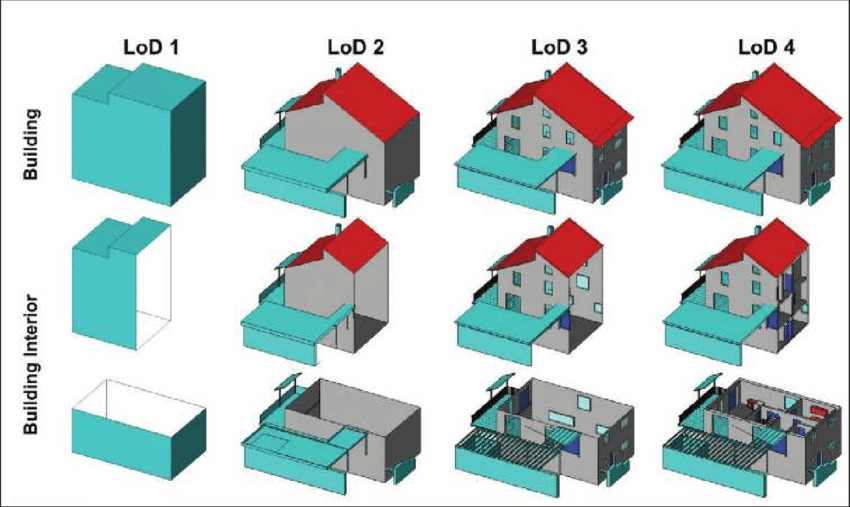
\includegraphics[width=0.8\textwidth]{images/LoD-for-building.png}}
				\caption {Different levels of detail (LoD) for buildings. Source: Karlsruhe Institute of Technology (KIT), CityGML 2.0 Encoding standard}
			\end{figure}
		}
	\end{frame}

	\begin{frame}{Заключение}
		Важность и выгоды использования Culling

		\begin{itemize}
			\item 	
			Экономия вычислительных ресурсов (процессор, GPU)
			\item 
			Уменьшение количества полигонов для рендеринга
			\item 
			Улучшение производительности в реальном времени (FPS)
		\end{itemize}

	\note{
		Оптимизация в движках. \\
		
		Компания Umbra Software была основана в 2006 году в Финляндии. Её цель --- разработка инструментов для оптимизации графики в реальном времени.
		
		Umbra --- коммерческая технология, разработанная для оптимизации рендеринга в реальном времени с акцентом на отсев (culling) невидимых объектов в сложных 3D-сценах. 

		Начиная с 2011 г., обновленная версия принесла значительные улучшения, включая поддержку огромных открытых миров. Технология стала широко использоваться в популярных игровых движках, таких как Unity и Unreal Engine. 

		Сегодня Umbra используется в современных играх, таких как
		The Witcher 3, Call of Duty, и Assassin's Creed и другие.

	}

	\end{frame}



	% \begin{frame}{Список использованной литературы}
		
	% \end{frame}

	\end{document}
	